

\documentclass{article}
% Template-specific packages

\usepackage{graphicx} % Required for including images
\usepackage[hidelinks]{hyperref}
\usepackage{longtable}
\usepackage{epstopdf}
\usepackage{fullpage,enumitem,amsmath,amssymb,graphicx}
\usepackage{tikz}
\usepackage{pdfpages}
\usepackage{amsmath, amsthm}
\usepackage{fancyhdr}
\usepackage{siunitx}
\usepackage{mathtools}
\usepackage{mathrsfs}
\newcommand{\slantbox}[2][0]{\mbox{%
        \sbox{\foobox}{#2}%
        \foodim=#1\wd\foobox
        \hskip \wd\foobox
        \hskip -0.5\foodim
        \pdfsave
        \pdfsetmatrix{1 0 #1 1}%
        \llap{\usebox{\foobox}}%
        \pdfrestore
        \hskip 0.5\foodim
}}
\def\Laplace{\slantbox[-.45]{\mathscr{L}}}
\pagestyle{fancy}
\fancyhead[R]{\rightmark}
\fancyhead[L]{Ali BaniAsad 401209244}
\setlength{\headheight}{10pt}
\setlength{\headsep}{0.2in}
\usepackage{titling}
\usepackage{float}
\newcommand\Tstrut{\rule{0pt}{2.6ex}}         % = `top' strut
\newcommand\Bstrut{\rule[-0.9ex]{0pt}{0pt}}   % = `bottom' strut
%----------------------------------------------------------------------------------------
%	ASSIGNMENT INFORMATION
%----------------------------------------------------------------------------------------



%----------------------------------------------------------------------------------------
\usepackage{graphicx}
\title{Home Work \#4}
\author{Ali BaniAsad 401209244}

\begin{document}
	\maketitle
	\section{Question 1}
We know inertia matrix is symetric so we have:
$$I_{xy} = I_{yx} = 10, \quad I_{xz} = I_{zx} = 0, \quad I_{yz} = I_{zy}$$

$$\boldsymbol{\mathrm{I}} = \begin{bmatrix}
    30 & -10 & 0 \\
    -10 & 20 & -I_{yz}\\
    0 & -I_{yz} & 30
\end{bmatrix}$$
\subsection{part a}
We know that:
\begin{equation}
    \boldsymbol{\mathrm{I}} \times \boldsymbol{\mathrm{\omega}} = \boldsymbol{\mathrm{h}}
\end{equation}

$$
\boldsymbol{\mathrm{\omega}} = \begin{bmatrix}
    10 & 10 & 10
\end{bmatrix}^T_{RPS} = \begin{bmatrix}
    10\times2\pi & 10\times2\pi & 10\times2\pi
\end{bmatrix}^T_{rad/\sec}, \quad \boldsymbol{\mathrm{h}} = \begin{bmatrix}
    200 & 200 & 400
\end{bmatrix}^T_{kg.m^2/s}
$$
If we use radian per second instead of revelotion per second $\boldsymbol{\mathrm{I}} \times \boldsymbol {\mathrm{\omega}} \neq \boldsymbol{\mathrm{h}}$ would happen.
$$ 
\boldsymbol{\mathrm{I}} \times \boldsymbol{\mathrm{\omega}} = \begin{bmatrix}
    200
    \\
    100 - 10I_{yz} \\
    300 - 10I_{yz}
\end{bmatrix} = \begin{bmatrix}
    200\\
    200\\
    400
\end{bmatrix} \rightarrow I_{yz} = -10 \rightarrow 
\boldsymbol{\mathrm{I}} = \begin{bmatrix}
    30 & -10 & 0 \\
    -10 & 20 & 10\\
    0 & 10 & 30
\end{bmatrix}
$$

\begin{equation}
T_{Rotational} = \dfrac{1}{2}\boldsymbol{\mathrm{\omega}}^T\times \boldsymbol{\mathrm{I}} \times \boldsymbol{\mathrm{\omega}} = \dfrac{1}{2} \begin{bmatrix}
    10&
    10&
    10
\end{bmatrix}\times
\begin{bmatrix}
    30 & -10 & 0 \\
    -10 & 20 & 10\\
    0 & 10 & 30
\end{bmatrix}\times
\begin{bmatrix}
    10\\
    10\\
    10
\end{bmatrix} = 4000
\end{equation}
\subsection{part b}
\begin{equation}
    T_{Rotational} = \dfrac{1}{2} \mathrm{I}_{\xi} \omega^2 \rightarrow \mathrm{I}_{\xi} = \dfrac{2T_{Rotational}}{\omega^2} = \dfrac{2\times 4000}{300} = 26.67
\end{equation}

Rotation matrix calculated via eigen vector of inertia matrix (used MATLAB to calculate).
\begin{equation}
    \boldsymbol{\mathrm{A}} = \mathrm{eig}(\boldsymbol{\mathrm{I}}) = \begin{bmatrix}
        -0.4082&   -0.7071&   -0.5774\\
        -0.8165&   -0.0000&    0.5774\\
         0.4082&   -0.7071&    0.5774\\
    \end{bmatrix}
\end{equation}
We know that above matrix shows the direction cosines of the principal axes with the primary body axes. Used MATLAB function (dcm2angle) to calculate euler angles between two corinate system.
$$
\begin{bmatrix}
    \phi\\
    \theta\\
    \psi 
\end{bmatrix} = \begin{bmatrix}
  \ang{45.00}\\
  \ang{35.26}\\
  \ang{-120.00}
\end{bmatrix}
$$

\subsection{part c}
Ellipsoid of inertia calculated as folow:
\begin{equation}
    \dfrac{X^2}{\left(\sqrt{\dfrac{1}{\mathrm{I}_x}}\right)^2} + 
    \dfrac{Y^2}{\left(\sqrt{\dfrac{1}{\mathrm{I}_y}}\right)^2} + 
    \dfrac{Z^2}{\left(\sqrt{\dfrac{1}{\mathrm{I}_z}}\right)^2} = 1
\end{equation} 

\begin{figure}[H]
    \caption{elipsoid of inertia}
    \centering
    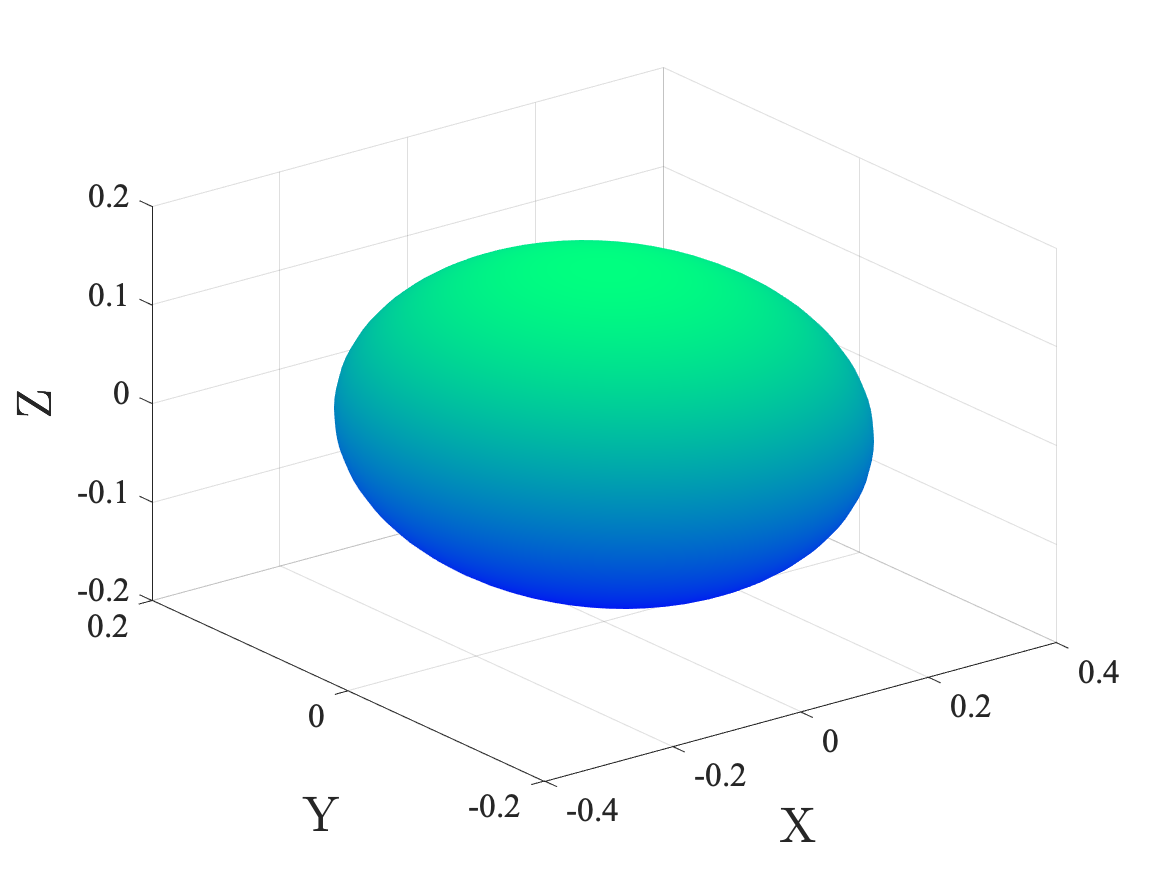
\includegraphics[width=17cm]{../Figure/Q1/3Dof_view_elipsoid_inertia}
\end{figure}

\begin{figure}[H]
    \caption{elipsoid of inertia in zx plane}
    \centering
    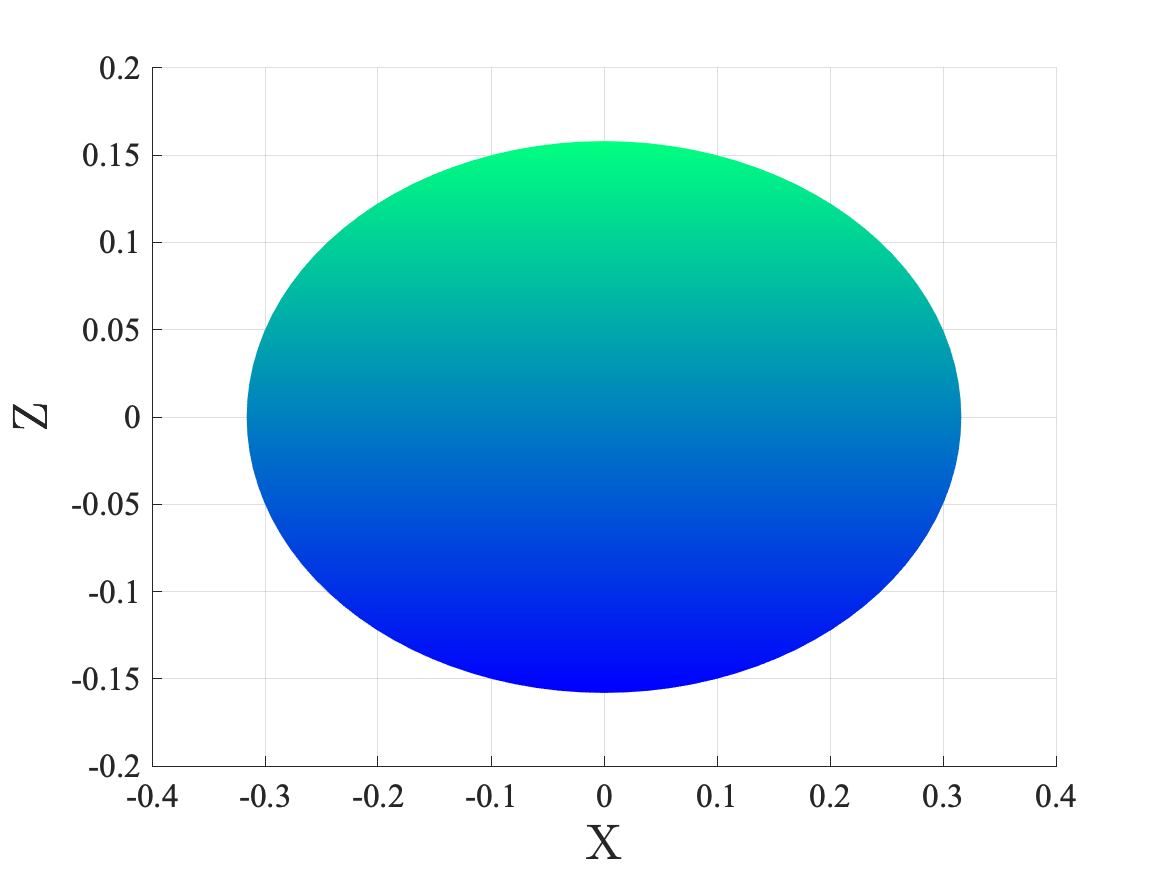
\includegraphics[width=12cm]{../Figure/Q1/xz_view_elipsoid_inertia}
\end{figure}

\begin{figure}[H]
    \caption{elipsoid of inertia zy plane}
    \centering
    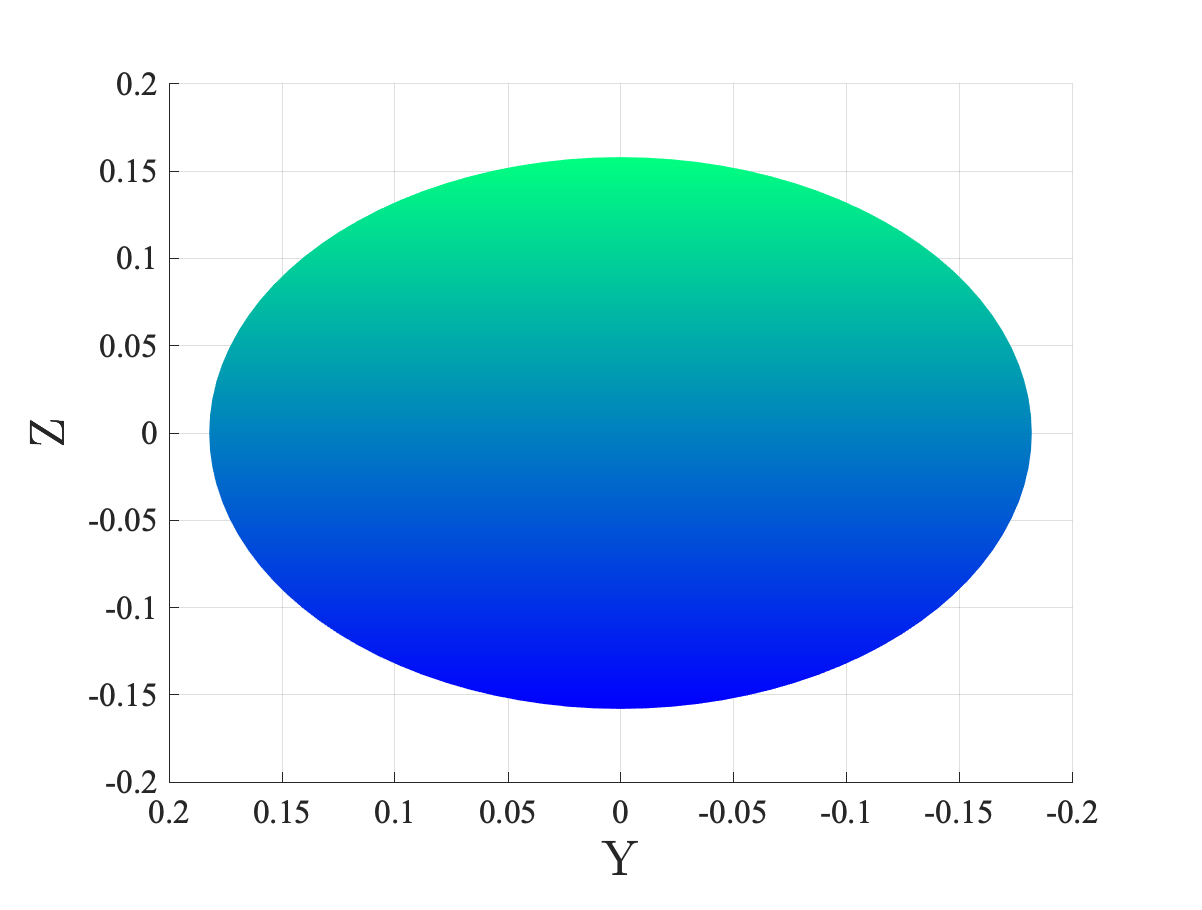
\includegraphics[width=12cm]{../Figure/Q1/yz_view_elipsoid_inertia}
\end{figure}

\begin{figure}[H]
    \caption{elipsoid of inertia in xy plane}
    \centering
    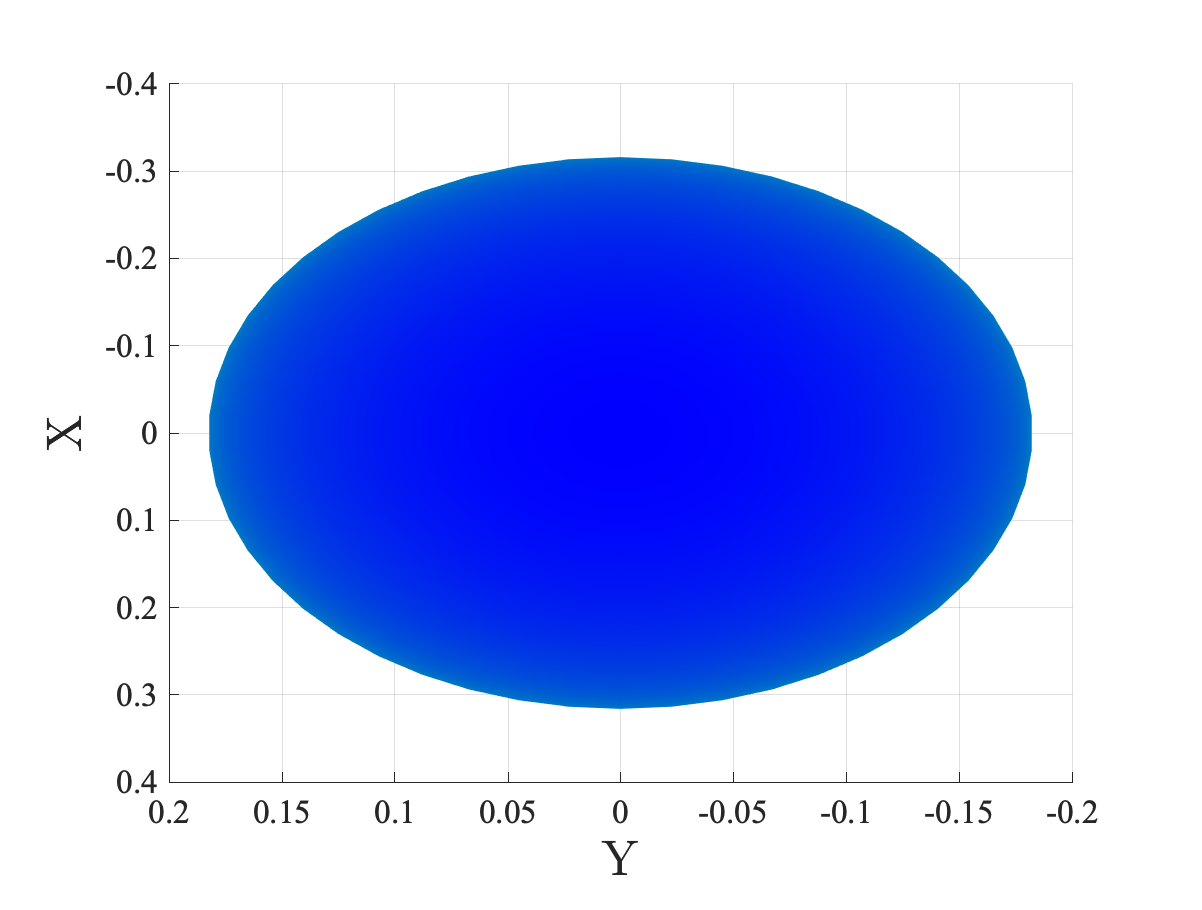
\includegraphics[width=12cm]{../Figure/Q1/xy_view_elipsoid_inertia}
\end{figure}
	\section{Question 2}
Data of the question:
$$
\mathrm{I}_x = 8_{kg.m^2},\quad \mathrm{I}_y = 10_{kg.m^2},\quad \mathrm{I}_z = 14_{kg.m^2}
$$
$$
\boldsymbol{\mathrm{q}}(0) = \begin{bmatrix}
    0.3 & 0.2 & 0.5 & 0.7874
\end{bmatrix}^T
$$

$$
\boldsymbol{\mathrm{\omega}}(0) = \begin{bmatrix}
    2 & 3 & -5
\end{bmatrix}^T \times 10^{-3}_{rps} = \begin{bmatrix}
    2\times 2\pi & 3\times 2\pi & -5\times 2\pi
\end{bmatrix}^T \times 10^{-3}_{rad/\sec}
$$

\section{part a}
Used MATLAB function(quat2eul) to calculate initial euler angles.
$$
\begin{bmatrix}
    \phi\\
    \theta\\
    \psi 
\end{bmatrix} = \begin{bmatrix}
  \ang{137.74}\\
  \ang{-0.86}\\
  \ang{65.16}
\end{bmatrix}
$$

\section{part b}
Equation of motion with gravity gradient:

\begin{align}
    I_x \dot\omega_x +  \omega_y \omega_z(I_z - I_y) = G_x\\
    I_y \dot\omega_y +  \omega_x \omega_z(I_x - I_z) = G_y\\
    I_z \dot\omega_z +  \omega_x \omega_y(I_y - I_x) = G_z\\
\end{align}

$$
\dot \omega_x = (G_x + \omega_y \omega_z(I_y - I_z))/I_x
$$

$$
\dot \omega_y = (G_y + \omega_x \omega_z(I_z - I_x))/I_y
$$

$$
\dot \omega_z = (G_z + \omega_y \omega_x(I_x - I_y))/I_z
$$

\begin{equation}
    \begin{bmatrix}
        \dot \omega_x \\
        \dot \omega_y \\
        \dot \omega_z
    \end{bmatrix} = \begin{bmatrix}
        p \\
        q \\
        r
    \end{bmatrix}  + \boldsymbol{\mathrm{C}}_R^b \begin{bmatrix}
        0 \\ -\omega_0 \\ 0
    \end{bmatrix} \to \begin{bmatrix}
        p \\
        q \\
        r
    \end{bmatrix} = \begin{bmatrix}
        \dot \omega_x \\
        \dot \omega_y \\
        \dot \omega_z
    \end{bmatrix} + \boldsymbol{\mathrm{C}}_R^b \begin{bmatrix}
        0 \\ \omega_0 \\ 0
    \end{bmatrix}
\end{equation}
where $\boldsymbol{\mathrm{C}}_R^b$ is transformation matrix.

\begin{equation}
    \boldsymbol{\mathrm{C}}_b^R = \begin{bmatrix}
        \cos(\theta)\cos(\psi) & -\cos(\phi)\sin(\psi) + \sin(\phi)\sin(\theta)\cos(\psi) & \sin(\phi)\sin(\psi) + \cos(\phi)\sin(\theta)\cos(\psi) \\
        \cos(\theta)\sin(\psi) & \cos(\phi)\cos(\psi) + \sin(\phi)\sin(\theta)\sin(\psi) & -\sin(\phi)\cos(\psi) + \cos(\phi)\sin(\theta)\sin(\psi) \\
        -\sin(\theta) & \sin(\phi)\cos(\theta) & \cos(\phi)\cos(\theta)
    \end{bmatrix}
\end{equation}


Using euler propagation:

\begin{equation}
    \begin{bmatrix}
        \dot \phi \\
        \dot \theta \\
        \dot \psi
    \end{bmatrix} = \begin{bmatrix}
        1 & \sin(\phi)\tan(\theta) & \cos(\phi)\tan(\theta)\\
        0 & \cos(\phi) & -\sin(\phi) \\
        0 & \dfrac{(\phi)}{\cos(\theta)} & \dfrac{\cos(\phi)}{\cos(\theta)}
    \end{bmatrix} \begin{bmatrix}
        p \\q \\ r
    \end{bmatrix}
\end{equation}

In linearized equation of motion we assume:

\begin{equation}
    \boldsymbol{\mathrm{C}}_b^R = \begin{bmatrix}
        1 & -\psi & \theta \\
        \psi & 1 & -\phi \\
        -\theta & \phi & 1
    \end{bmatrix}, \quad \begin{bmatrix}
        p \\ q \\ r
    \end{bmatrix} = \begin{bmatrix}
        \dot \phi \\
        \dot \theta \\
        \dot \psi
    \end{bmatrix}
\end{equation}

For the transformation from reference to body use the transpose of the desciberd matrix above.


The equations of motions solved in MATLAB with ode45 function. Below is the figure of euler angles simulation in 50 and 1000 seconds.

\begin{figure}[H]
    \caption{simulation of $\phi$ for 50 seconds}
    \centering
    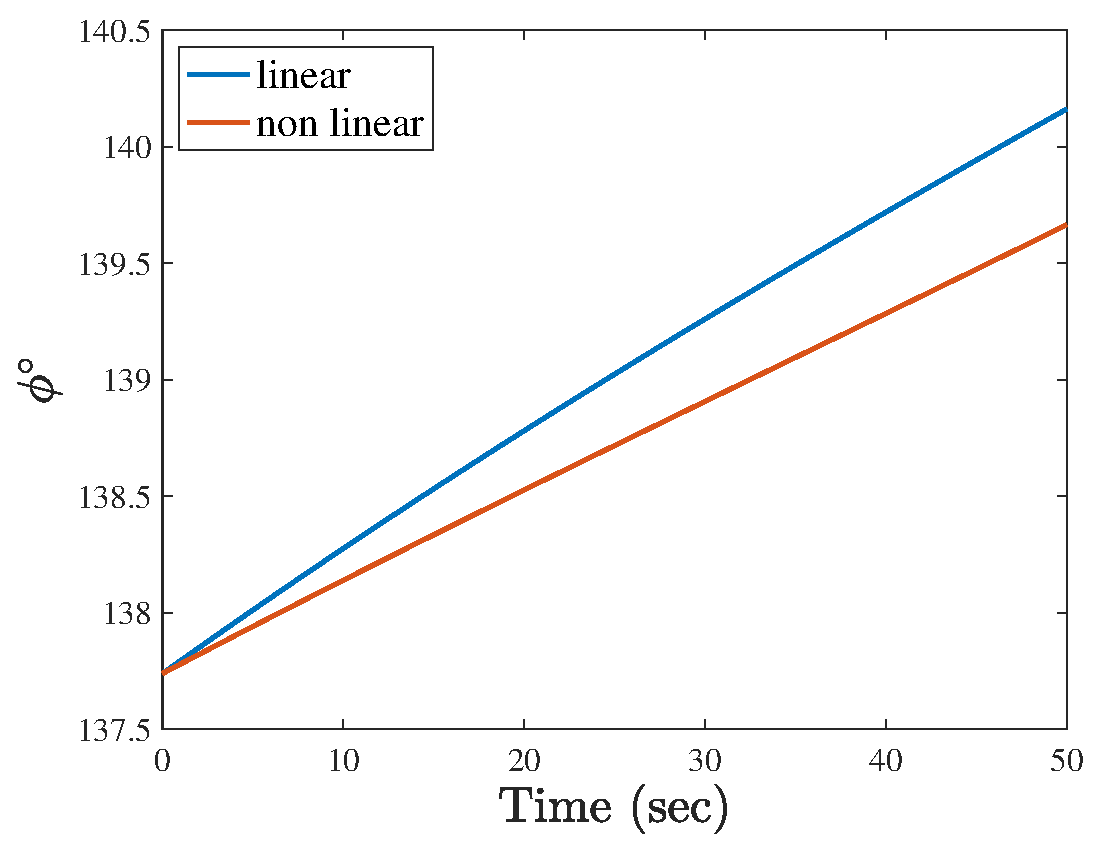
\includegraphics[width=12cm]{../Figure/Q2/phi_50}
\end{figure}

\begin{figure}[H]
    \caption{simulation of $\theta$ for 50 seconds}
    \centering
    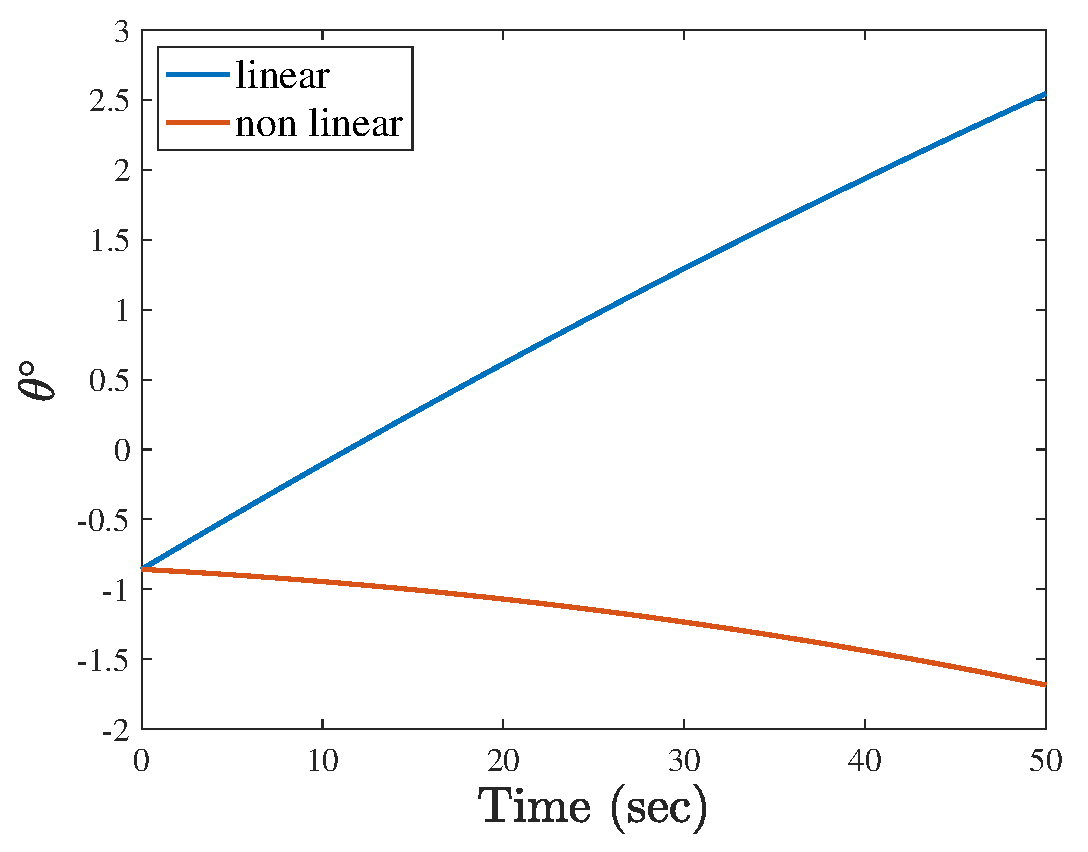
\includegraphics[width=12cm]{../Figure/Q2/theta_50}
\end{figure}

\begin{figure}[H]
    \caption{simulation of $\psi$ for 50 seconds}
    \centering
    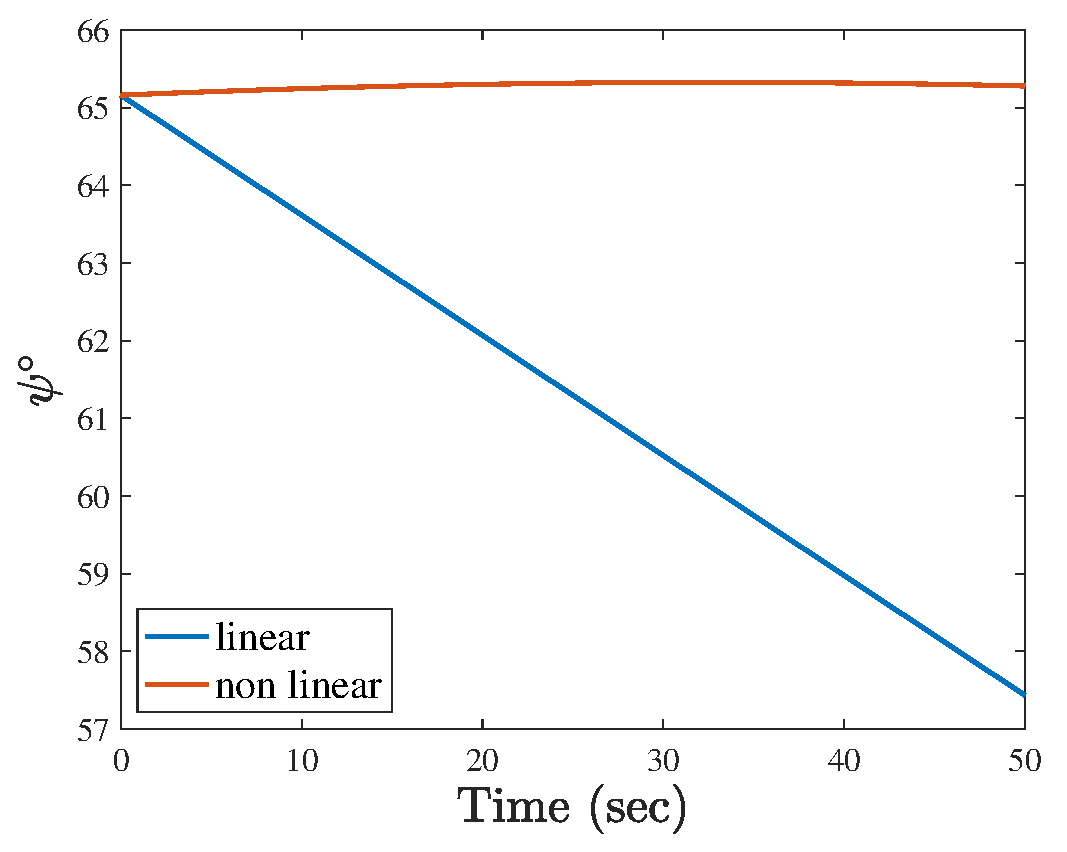
\includegraphics[width=12cm]{../Figure/Q2/psi_50}
\end{figure}

%%%%%%%%%% 1000 %%%%%%%%%%
\begin{figure}[H]
    \caption{simulation of $\phi$ for 5000 seconds}
    \centering
    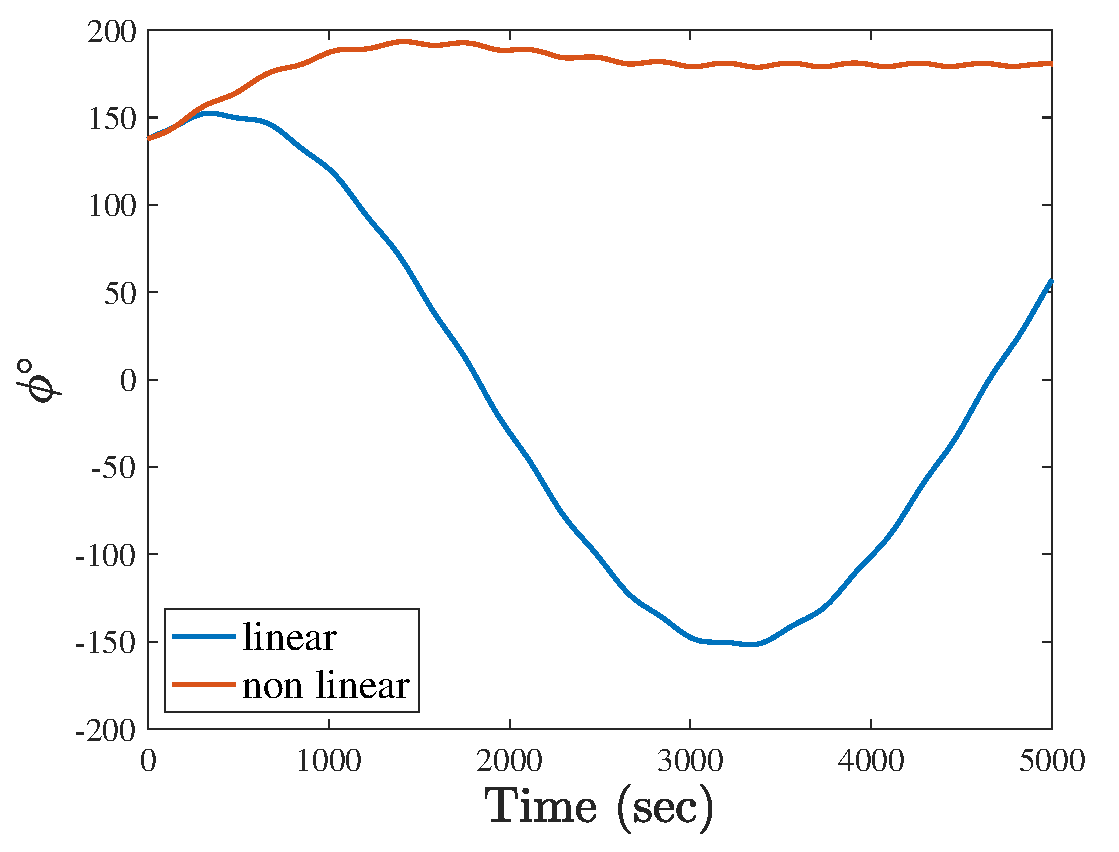
\includegraphics[width=12cm]{../Figure/Q2/phi_5000}
\end{figure}

\begin{figure}[H]
    \caption{simulation of $\theta$ for 5000 seconds}
    \centering
    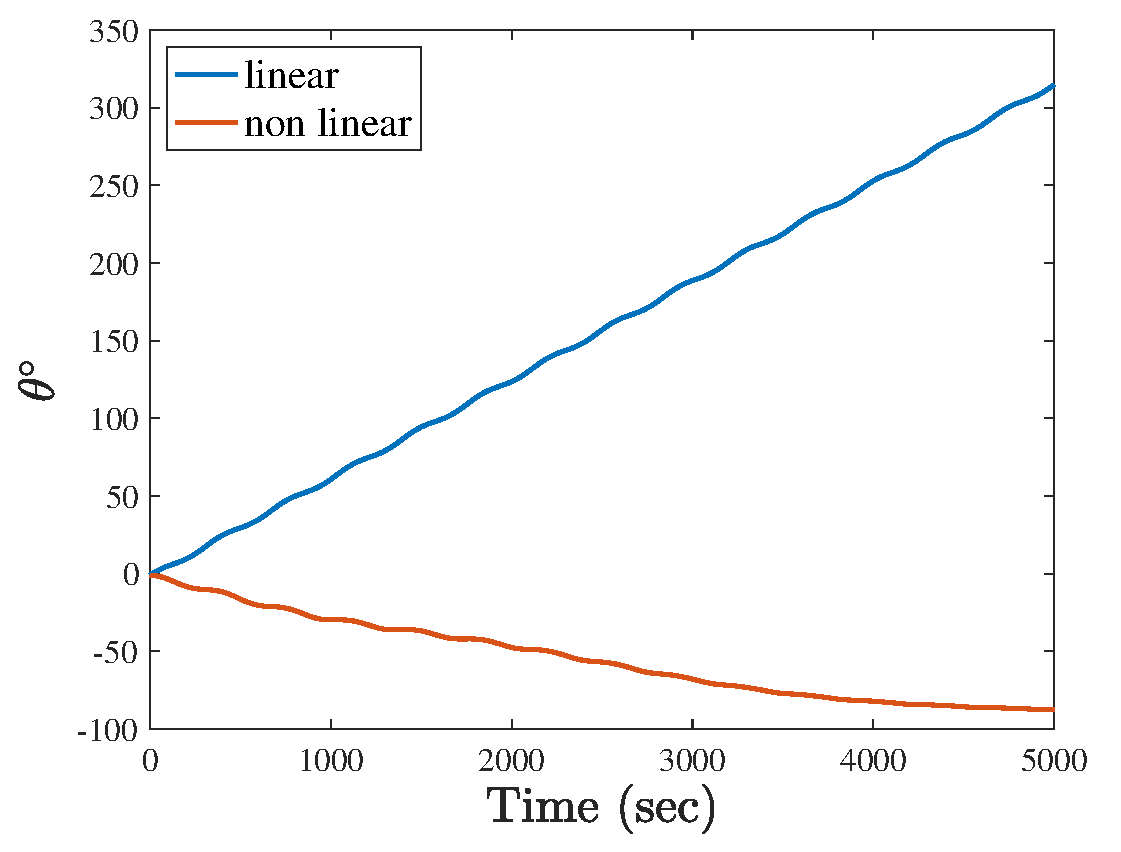
\includegraphics[width=12cm]{../Figure/Q2/theta_5000}
\end{figure}

\begin{figure}[H]
    \caption{simulation of $\psi$ for 5000 seconds}
    \centering
    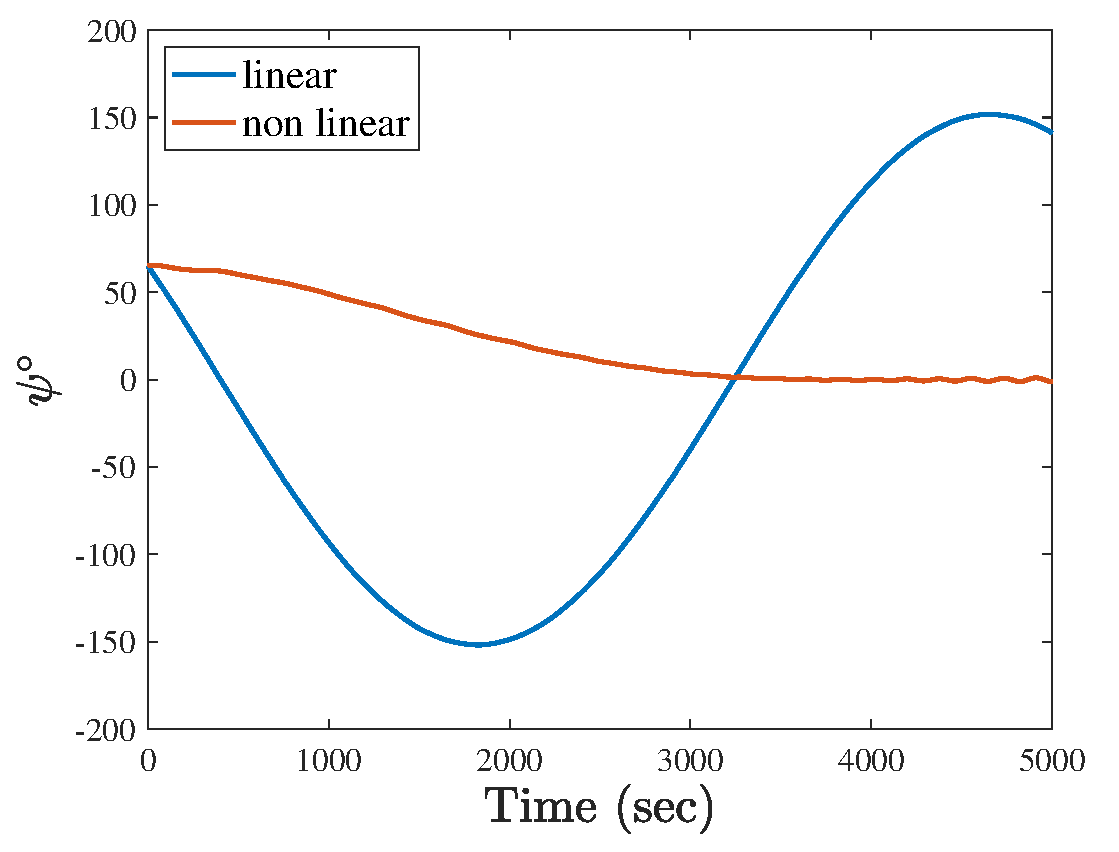
\includegraphics[width=12cm]{../Figure/Q2/psi_5000}
\end{figure}

\section{part d}

Used above equation with different initial conditions and add initial torque disturbance.

\begin{figure}[H]
    \caption{simulation of $\phi$ with torque disturbance}
    \centering
    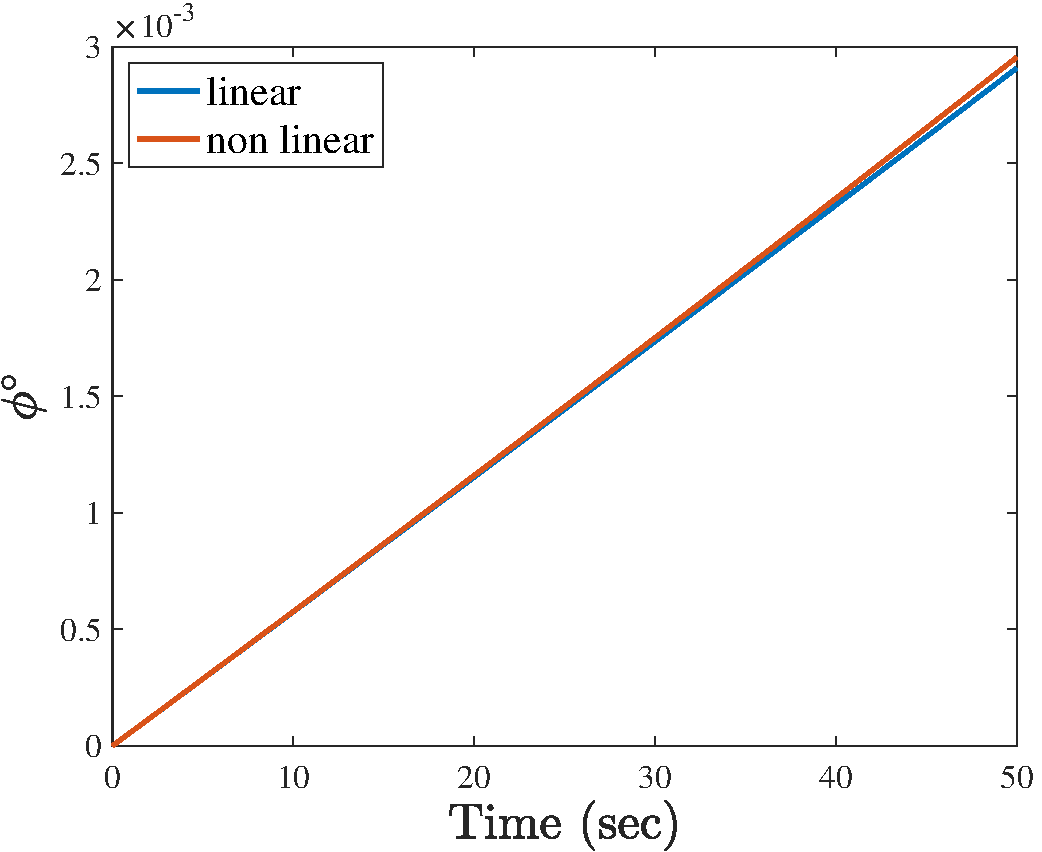
\includegraphics[width=12cm]{../Figure/Q2/phi_part_d}
\end{figure}

\begin{figure}[H]
    \caption{simulation of $\theta$ with torque disturbance}
    \centering
    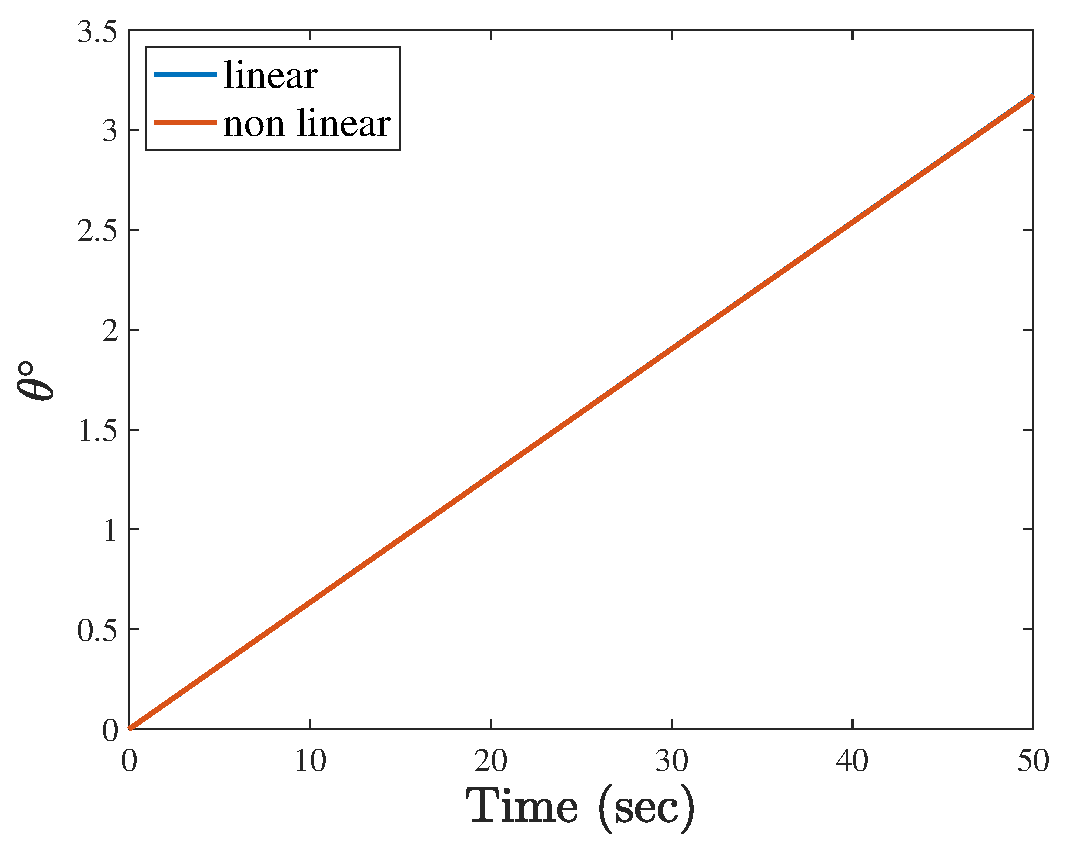
\includegraphics[width=12cm]{../Figure/Q2/theta_part_d}
\end{figure}

\begin{figure}[H]
    \caption{simulation of $\psi$ with torque disturbance}
    \centering
    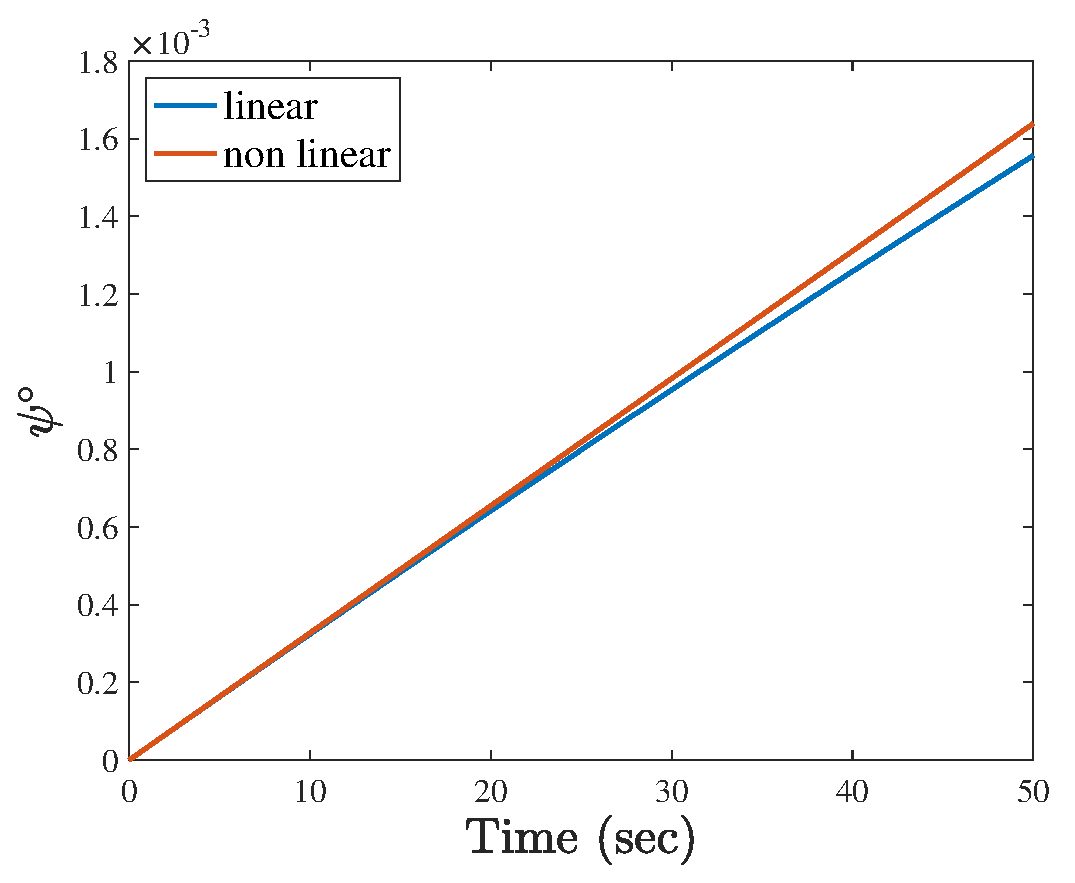
\includegraphics[width=12cm]{../Figure/Q2/psi_part_d}
\end{figure}

	\section{Question 3}

	\newpage
	\tableofcontents
	\newpage
	\listoffigures
	% \newpage
	% \listoftables
\end{document}

